\documentclass[12pt]{article}
\usepackage[a4paper,margin=1in]{geometry}
\usepackage{amsmath}
\usepackage{amssymb}
\usepackage{enumitem}
\usepackage{tikz}
\usetikzlibrary{
    arrows.meta,
    calc,
    angles,
    quotes,
    decorations.pathmorphing
}
\usepackage[american]{circuitikz}


\begin{document}

\begin{enumerate}

\item One mole of a monoatomic ideal gas $(\gamma = 5/3)$ initially at state $(P_0,V_0,T_0)$ undergoes a fully reversible cyclic process. First it expands isothermally at temperature $T_0$ until its volume becomes $V_1 = 243V_0$. From this state it undergoes adiabatic expansion until its temperature falls to $T_0/81$. The gas is then compressed isothermally at temperature $T_0/81$ until it reaches a state that lies exactly on the adiabatic curve passing through the original state $(P_0,V_0,T_0)$. Finally it is compressed adiabatically back to the initial state.

You are required to determine the exact intermediate volume reached during the third process using $TV^{\gamma-1}=\text{constant}$, and then evaluate the net work per cycle without assuming symmetry of enclosed areas. Express the final answer entirely in terms of $RT_0$.

% Diagram for Question 1

\begin{center}
\textbf{Diagram for Question 1}
\end{center}

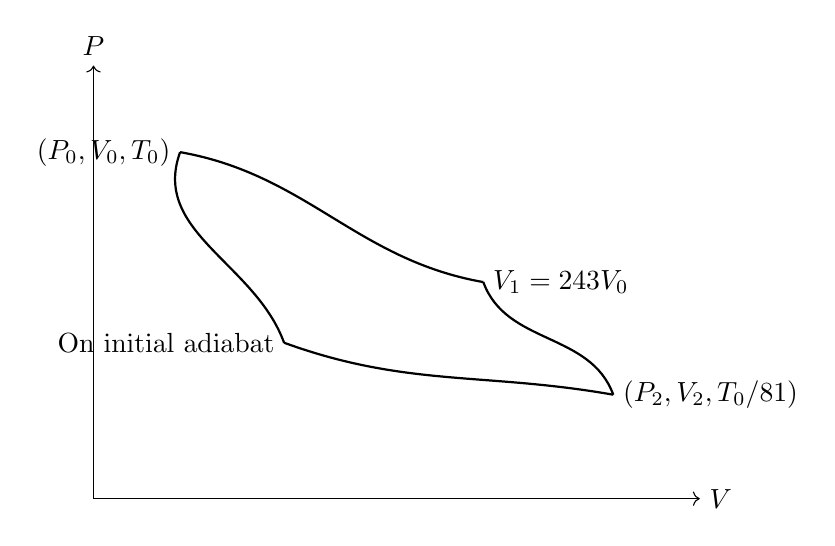
\begin{tikzpicture}[scale=1.1]

% Axes
\draw[->] (0,0) -- (7,0) node[right] {$V$};
\draw[->] (0,0) -- (0,5) node[above] {$P$};

% Points
\coordinate (A) at (1,4);
\coordinate (B) at (4.5,2.5);
\coordinate (C) at (6,1.2);
\coordinate (D) at (2.2,1.8);


% Curves (isothermal and adiabatic with correct steepness distinction)
\draw[thick] (A) to[out=-10,in=170] (B);      % isothermal (gentler)
\draw[thick] (B) to[out=-70,in=110] (C);     % adiabatic (steeper)
\draw[thick] (C) to[out=170,in=-20] (D);     % isothermal (gentler)
\draw[thick] (D) to[out=110,in=-110] (A);    % adiabatic (steeper)

% Labels
\node[left] at (A) {$(P_0,V_0,T_0)$};
\node[right] at (B) {$V_1=243V_0$};
\node[right] at (C) {$(P_2,V_2,T_0/81)$};
\node[left] at (D) {On initial adiabat};

\end{tikzpicture}

(A) $RT_0 \ln 243 \left(1-81^{-1/3}\right)$  

(B) $RT_0 \ln 243 \left(1-81^{-2/3}\right)$  

(C) $\frac{2}{3}RT_0 \ln 243$  

(D) $RT_0 \ln 9 \left(1-9^{-4/3}\right)$  

\item A monoatomic ideal gas is compressed reversibly and adiabatically from state $(P_0,V_0,T_0)$ to a final pressure $P_f = 3^{15}P_0$. The mean free path varies as $\lambda \propto \dfrac{T}{P}$ and the rms speed varies as $v_{rms}\propto \sqrt{T}$. Collision frequency is defined as $f=\dfrac{v_{rms}}{\lambda}$.

Using exact exponent tracking through the relation $T\propto P^{(\gamma-1)/\gamma}$, determine the power $n$ such that $\dfrac{f_f}{f_i}=3^{n}$.

(A) 8  

(B) 9  

(C) 10  

(D) 11  

\item In Young’s double slit experiment the slit separation is $d$, screen distance is $D$, and wavelength in air is $\lambda$. A transparent slab of thickness $t$ and refractive index $\mu$ is placed in front of one slit. The entire arrangement is then immersed in a liquid of refractive index $\mu$. Finally the screen is rotated by a small angle $\theta$ so that the effective fringe spacing changes geometrically and small-angle approximation must be used consistently.

If original fringe width in air is $\beta=\dfrac{\lambda D}{d}$, determine the shift of central maximum in terms of $\beta$ after accounting simultaneously for optical path difference, wavelength reduction in medium, and geometric projection due to screen tilt.

% Diagram for Question 3

\begin{center}
\textbf{Diagram for Question 3}
\end{center}

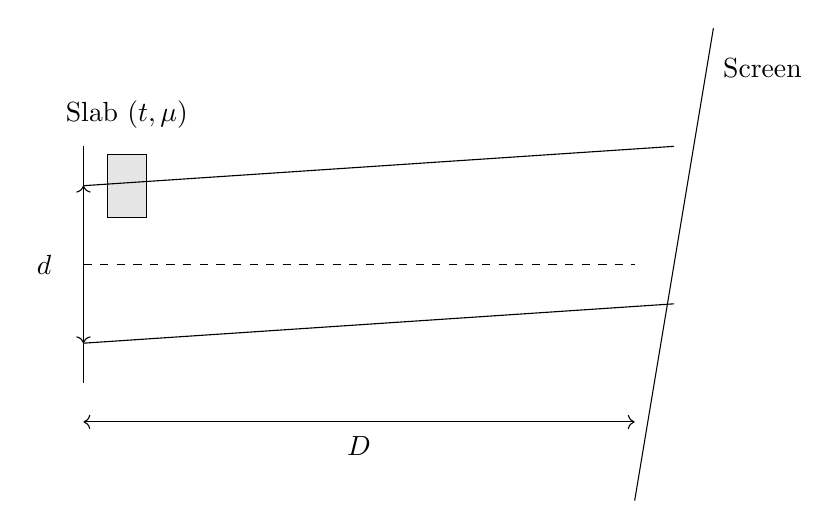
\begin{tikzpicture}[scale=1]

% Slits
\draw (-1,0.5) -- (-1,1.5);
\draw (-1,-1.5) -- (-1,-0.5);

% Slab
\draw[fill=gray!20] (-0.7,0.6) rectangle (-0.2,1.4);
\node at (-0.45,1.9) {Slab $(t,\mu)$};

% Central axis
\draw[dashed] (-1,0) -- (6,0);

% Screen tilted
\draw (6,-3) -- (7,3);
\node[right] at (7,2.5) {Screen};

% Rays
\draw (-1,1) -- (6.5,1.5);
\draw (-1,-1) -- (6.5,-0.5);

% Distance labels
\draw[<->] (-1,-2) -- (6,-2);
\node at (2.5,-2.3) {$D$};

\draw[<->] (-1,-1) -- (-1,1);
\node at (-1.5,0) {$d$};

\end{tikzpicture}

(A) $\dfrac{(\mu-1)t}{\mu\lambda}\beta$  

(B) $\dfrac{(\mu-1)t}{\lambda}\beta$  

(C) $\dfrac{t}{\mu\lambda}\beta$ 

(D) Zero  

\item A closed organ pipe of length $L$ contains gas whose temperature varies along its length according to  

\[
T(x)=T\left(1+120\frac{x}{L}+256\frac{x^2}{L^2}\right)
\]

The local speed of sound is $v(x)=\sqrt{\gamma RT(x)/M}$. The fundamental mode must satisfy  

\[
\int_0^L \frac{dx}{v(x)}=\frac{1}{4f}
\]

Perform the integration exactly (no binomial approximation permitted) and determine the ratio $\dfrac{f}{f_0}$, where $f_0$ is the frequency for uniform temperature $T$.

% Diagram for Question 4

\begin{center}
\textbf{Diagram for Question 4}
\end{center}

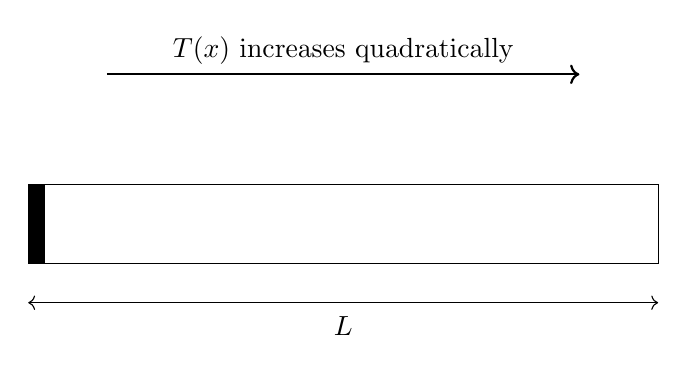
\begin{tikzpicture}[scale=1]

% Pipe
\draw (0,0) rectangle (8,1);

% Closed end
\draw[fill=black] (0,0) rectangle (0.2,1);

% Open end
\draw (8,0) -- (8,1);

% Length label
\draw[<->] (0,-0.5) -- (8,-0.5);
\node at (4,-0.8) {$L$};

% Temperature gradient arrow
\draw[->,thick] (1,2.4) -- (7,2.4);
\node at (4,2.7) {$T(x)$ increases quadratically};

\end{tikzpicture}

(A) 8  

(B) 10  

(C) 12  

(D) 16  

\item An incompressible, non-viscous liquid flows steadily through a horizontal pipe. The radius decreases successively from $R$ to $R/5$, and then from $R/5$ to $R/25$. The initial velocity is $v_0$. Continuity must be applied at each stage and Bernoulli’s equation must be used stepwise, not by directly comparing initial and final areas.

Determine the final pressure drop $P_0-P_f$ in terms of $\rho v_0^2$.

% Diagram for Question 5

\begin{center}
\textbf{Diagram for Question 5}
\end{center}

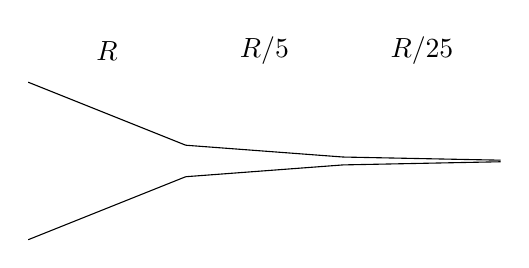
\begin{tikzpicture}[scale=1]

% First section (R)
\draw (0,0) -- (2,0.8);
\draw (0,2) -- (2,1.2);

% Second section (R/5)
\draw (2,0.8) -- (4,0.95);
\draw (2,1.2) -- (4,1.05);

% Third section (R/25)
\draw (4,0.95) -- (6,0.99);
\draw (4,1.05) -- (6,1.01);

% Labels
\node at (1,2.4) {$R$};
\node at (3,2.4) {$R/5$};
\node at (5,2.4) {$R/25$};

\end{tikzpicture}

(A) $\dfrac{390624}{2}\rho v_0^2$ 

(B) $390624\rho v_0^2$  

(C) $\dfrac{390625}{2}\rho v_0^2$  

(D) $390625\rho v_0^2$  

\item A particle of mass $m$ executes SHM with amplitude $A$. When its displacement is $x=\dfrac{9A}{10}$ and it is moving toward the mean position, the spring constant suddenly increases from $k$ to $196k$. Displacement and velocity remain continuous during the change.

Using full reconstruction of total mechanical energy immediately before and after the change (without assuming amplitude symmetry), determine the new amplitude $A'$.

% Diagram for Question 6

\begin{center}
\textbf{Diagram for Question 6}
\end{center}

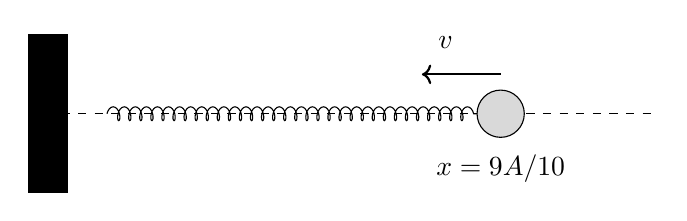
\begin{tikzpicture}[scale=1]

% Equilibrium line
\draw[dashed] (0,0) -- (8,0);

% Mass at position
\draw[fill=gray!30] (6,0) circle (0.3);
\node at (6,-0.7) {$x=9A/10$};

% Spring
\draw[decorate,decoration={coil,aspect=0.5,segment length=4pt}] (1,0) -- (5.7,0);


% Wall
\draw[fill=black] (0, -1) rectangle (0.5,1);

% Arrow toward mean
\draw[->,thick] (6,0.5) -- (5,0.5);
\node at (5.3,0.9) {$v$};

\end{tikzpicture}

(A) $\dfrac{A}{14}\sqrt{19601}$  

(B) $\dfrac{A}{14}\sqrt{18001}$ 

(C) $\dfrac{A}{14}\sqrt{16201}$  

(D) $\dfrac{A}{14}\sqrt{20001}$  

\item A Carnot engine operates between reservoirs at $T_H$ and $T_C=\dfrac{T_H}{64}$. In engine mode it absorbs heat $Q_H$ and produces work $W_E$. The engine is then reversed and used as a refrigerator between the same reservoirs. However, the work input per cycle in refrigerator mode is 25 times the work output in engine mode.

Determine the ratio $\dfrac{Q_{C,\text{refrigerator}}}{Q_H}$.

(A) $\dfrac{25}{63}$ 

(B) $\dfrac{25}{64}$  

(C) $\dfrac{25}{4032}$  

(D) $\dfrac{25}{3969}$  

\item A diatomic gas $(\gamma=7/5)$ expands reversibly and adiabatically so that its pressure decreases to $P_f=2^{-42}P_i$. Using the relations $T\propto P^{(\gamma-1)/\gamma}$ and $v_{rms}\propto\sqrt{T}$, determine exponent $n$ such that $\dfrac{v_f}{v_i}=2^{-n}$.

(A) 5  

(B) 6  

(C) 7  

(D) 8  

\item A thin convex lens of refractive index $n$ has focal length $f$ in air given by  

\[
\frac{1}{f}=(n-1)\Phi
\]

When immersed in a liquid of refractive index $\mu$, its focal length becomes  

\[
\frac{1}{f'}=\left(\frac{n}{\mu}-1\right)\Phi
\]

Derive expression for $\dfrac{f'}{f}$ and determine the precise algebraic condition under which the lens changes from converging to diverging.

% Diagram for Question 9

\begin{center}
\textbf{Diagram for Question 9}
\end{center}

\begin{tikzpicture}[scale=1]


% Lens
\draw[thick] (3,-2) .. controls (2.6,0) .. (3,2);
\draw[thick] (3,-2) .. controls (3.4,0) .. (3,2);

% Medium box
\draw[dashed] (1,-3) rectangle (6,3);
\node at (4.8,2.4) {Medium $\mu$};

% Optical axis
\draw[dashed] (0,0) -- (8,0);

\node at (4.2,1.2) {$n$};

\end{tikzpicture}

(A) $\dfrac{f'}{f}=\dfrac{n-1}{\frac{n}{\mu}-1}$, sign change if $n<\mu$  

(B) $\dfrac{f'}{f}=\dfrac{\frac{n}{\mu}-1}{n-1}$, sign change if $n>\mu$  

(C) $\dfrac{f'}{f}=\dfrac{n-\mu}{n-1}$, sign change if $n<1$  

(D) $\dfrac{f'}{f}=\dfrac{n-1}{n-\mu}$, sign change if $n>\mu$  

\item A soap bubble of initial radius $R$ is expanded slowly and isothermally until its radius becomes $128R$. The excess pressure inside is $\Delta P=\dfrac{4T}{R}$. During expansion, one must account simultaneously for work done in increasing internal gas volume, work done against atmospheric pressure, and increase in surface energy of both surfaces of the bubble.

Derive the total work done and express it in the form $W=k\pi TR^2$. Determine $k$.

% Diagram for Question 10

\begin{center}
\textbf{Diagram for Question 10}
\end{center}

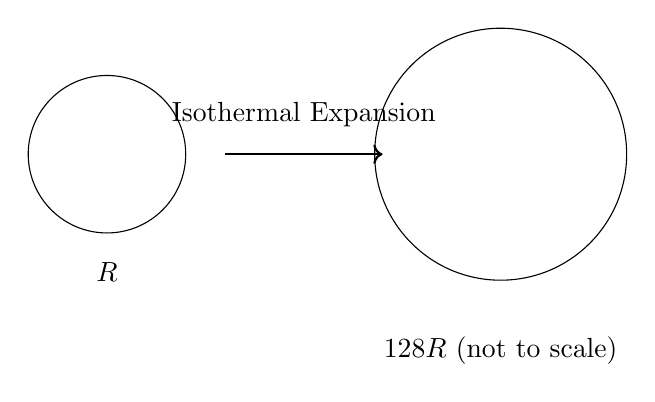
\begin{tikzpicture}[scale=1]

% Initial bubble
\draw (0,0) circle (1);
\node at (0,-1.5) {$R$};

% Final bubble
\draw (5,0) circle (1.6);
\node at (5,-2.5) {$128R$ (not to scale)};

% Arrow
\draw[->,thick] (1.5,0) -- (3.5,0);
\node at (2.5,0.5) {Isothermal Expansion};

\end{tikzpicture}

(A) 524288 

(B) 589824 

(C) 655360  

(D) 720896  

\item For an ideal gas at state $(P,V)$, both isothermal and adiabatic curves pass through that point. Using explicit differentiation of $PV=RT$ and $PV^\gamma=\text{constant}$, compute exactly  

\[
\left|\frac{(dP/dV)_S}{(dP/dV)_T}\right|
\]

without using remembered shortcut results.

(A) $\gamma$  

(B) $\gamma^2$  

(C) $1/\gamma$  

(D) $\sqrt{\gamma}$  

\item In an ideal gas, temperature increases by 600\%, molecular mass decreases by 36\%, and $\gamma$ increases by 44\%. Using $v=\sqrt{\frac{\gamma RT}{M}}$, determine the percentage increase in speed.

(A) 250\%  

(B) 300\%  

(C) 350\%  

(D) 400\%  

\item For laminar flow $Q\propto\dfrac{r^4\Delta P}{\eta L}$. Suppose radius decreases by $x\%$, pressure difference increases by $6x\%$, viscosity increases by $2x\%$, and length increases by $x\%$, where $x\ll100$. Using first-order binomial expansion and retaining only linear terms in $x$, determine net percentage change in $Q$.

(A) $-x\%$ 

(B) $-2x\%$  

(C) 0  

(D) $+x\%$  

\item A particle executing SHM has amplitude increased by small fraction $\varepsilon$ while angular frequency decreases by $5\varepsilon$. Using $E=\frac12 m\omega^2A^2$ and retaining only first-order terms in $\varepsilon$, determine fractional change in total mechanical energy.

(A) $-8\varepsilon$  

(B) $-6\varepsilon$  

(C) $-4\varepsilon$  

(D) 0  

\item A perfect black body obeys Wien’s displacement law $\lambda_{max}T=\text{constant}$ and Stefan’s law $P\propto T^4$. If temperature increases by a small fraction $\varepsilon$, determine the fractional change in peak frequency $\nu_{max}$ using $\nu_{max}=\dfrac{c}{\lambda_{max}}$. Work to first order in $\varepsilon$ and avoid substituting memorized proportionalities directly without derivation.

(A) $+\varepsilon$  

(B) $-\varepsilon$  

(C) $4\varepsilon$  

(D) 0  

\end{enumerate}

\end{document}